\documentclass[10pt,twoside]{article}
\usepackage[utf8]{inputenc}
\usepackage{amsmath}
\usepackage{amsfonts}
\usepackage{amssymb}
\usepackage[spanish,es-noshorthands]{babel}
\usepackage[T1]{fontenc}
\usepackage{lmodern}
\usepackage{graphicx,hyperref}
\usepackage{tikz,pgf}
\usepackage{multicol}
\usepackage{subfig}
\usepackage[papersize={6.5in,8.5in},width=5.5in,height=7in]{geometry}
\usepackage{fancyhdr}
\pagestyle{fancy}
\fancyhead[LE]{
\includegraphics[height=12pt]{Images/logo-colegio.png} Cálculo $11^{\circ}$}
\fancyhead[RE]{}
\fancyhead[RO]{\textit{Germ\'an Avenda\~no Ram\'irez, Lic. U.D., M.Sc. U.N.}}
\fancyhead[LO]{}

\author{Germ\'an Avenda\~no Ram\'irez, Lic. U.D., M.Sc. U.N.}
\title{\begin{minipage}{.2\textwidth}

\includegraphics[height=1.75cm]{Images/logo-colegio.png}\end{minipage}
\begin{minipage}{.55\textwidth}
\begin{center}
Taller, Calculando límites algebraicamente\\
Cálculo $11^{\circ}$
\end{center}
\end{minipage}\hfill
\begin{minipage}{.2\textwidth}

\includegraphics[height=1.75cm]{Images/logo-sed.png} 
\end{minipage}}
\date{}
\begin{document}
\maketitle
Nombre: \hrulefill Curso: \underline{\hspace*{44pt}} Fecha: \underline{\hspace*{2.5cm}}
\section*{Propiedades de los l\'{i}mites}
Para resolver l\'{i}mites algebraicamente, es necesario y \'{u}til aplicar sus propiedades:
\begin{enumerate}
\item $\displaystyle{\lim_{x \rightarrow a}[f(x)+g(x)]=\lim_{x \rightarrow a}f(x)+\lim_{x\rightarrow a}g(x)}$ \hfill Límite de una suma
\item $\displaystyle{\lim_{x\rightarrow a}[f(x)-g(x)]=\lim_{x\rightarrow a}f(x)-\lim_{x\rightarrow a}g(x)}$ \hfill Límite de una diferencia
\item $\displaystyle{\lim_{x\rightarrow a}[cf(x)]=c\lim_{x\rightarrow a}f(x)}$ \hfill Límite de una constante por una función
\item $\displaystyle{\lim_{x\rightarrow a}[f(x)g(x)]=\lim_{x\rightarrow a}f(x)\cdot \lim_{x\rightarrow a}g(x)}$ \hfill Límite del producto
\item $\displaystyle{\lim_{x\rightarrow a}\dfrac{f(x)}{g(x)}}=\dfrac{\displaystyle{\lim_{x\rightarrow a}}f(x)}{\displaystyle{\lim_{x\rightarrow a}}g(x)} \qquad \text{si} \qquad \displaystyle{\lim_{x\rightarrow a}g(x)\neq 0}$ \hfill Límite de un cociente

Estas propiedades las aplicamos al resolver un límite de una función polinómica o racional. Además de éstas propiedades, también tenemos las siguientes propiedades especiales, algunas aplicadas a la potenciación y la radicación:
\item $\displaystyle{\lim_{x\rightarrow a}}c=c$
\item $\displaystyle{\lim_{x\rightarrow a}}x=a$
\item $\displaystyle{\lim_{x\rightarrow a}}x^{n}=a^{n}$ \hspace*{1cm} Para $n$ entero positivo
\item $\displaystyle{\lim_{x\rightarrow a}}\sqrt[n]{x}=\sqrt[n]{a}$ \hspace*{1cm} Para $n$ entero positivo y $a>0$
\end{enumerate}
\paragraph*{Ejemplos:} Resolver los límites siguientes: 
\begin{enumerate}
\item $\displaystyle{\lim_{x\rightarrow 5}}(2x^{2}-3x+4$
\item $\displaystyle{\lim_{x\rightarrow -2}}\dfrac{x^{3}+2x^{2}-1}{5-3x}$
\end{enumerate}
\subparagraph*{Solución:}
\subsection*{Taller}
\begin{enumerate}
\item Suponga que:
\begin{tabbing}
\hspace{3cm}\=\hspace{3cm}\=\kill
$\displaystyle{\lim_{x\rightarrow a}}f(x)=-3$ \> $\displaystyle{\lim_{x\rightarrow a}}g(x)=0$ \> $\displaystyle{\lim_{x\rightarrow a}}h(x)=8$
\end{tabbing} 
Encuentre los valores de los l\'{i}mites. Si el l\'{i}mite no existe, explique por qu\'{e}
\begin{enumerate}
\begin{multicols}{3}
\item $\displaystyle{\lim_{x\rightarrow a}}[f(x)+g(x)]$
\item $\displaystyle{\lim_{x\rightarrow a}}[f(x)]^{2}$
\item $\displaystyle{\lim_{x\rightarrow a}}\sqrt[3]{h(x)}$
\item $\displaystyle{\lim_{x\rightarrow a}}\dfrac{f(x)}{h(x)}$
\item $\displaystyle{\lim_{x\rightarrow a}}\dfrac{1}{f(x)}$
\item $\displaystyle{\lim_{x\rightarrow a}}\dfrac{g(x)}{f(x)}$
\item $\displaystyle{\lim_{x\rightarrow a}}\dfrac{f(x)}{g(x)}$
\item $\displaystyle{\lim_{x\rightarrow a}}\dfrac{2f(x)}{h(x)-f(x)}$
\end{multicols}
\end{enumerate}
\item Observe las gráficas de $f$ y $g$. Úselas para evaluar cada límite si existe. Si no existe, explique por qué.
\begin{center}
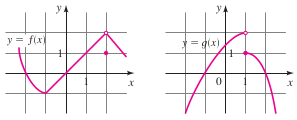
\includegraphics[scale=.8]{Images/funciones_fyg.png} 
\end{center}
\begin{enumerate}
\begin{multicols}{2}
\item $\displaystyle{\lim_{x\rightarrow 2}}[f(x)+g(x)]$
\item $\displaystyle{\lim_{x\rightarrow 1}}[f(x)+g(x)]$
\item $\displaystyle{\lim_{x\rightarrow 0}}[f(x)g(x)]$
\item $\displaystyle{\lim_{x\rightarrow -1}}\dfrac{f(x)}{g(x)}$
\item $\displaystyle{\lim_{x\rightarrow 2}}x^{3}f(x)$
\item $\displaystyle{\lim_{x\rightarrow 1}}\sqrt{3+f(x)}$
\end{multicols}
\end{enumerate}
Evalúe el límite justificando cada paso con el uso de las propiedades.
\begin{multicols}{2}
\item $\displaystyle{\lim_{x\rightarrow 4}}(5x^{2}-2x+3$
\item $\displaystyle{\lim_{x\rightarrow 3}}(x^{3}+2)(x^{2}-5x)$
\item $\displaystyle{\lim_{x\rightarrow -1}}\dfrac{x-2}{x^{2}+4x-3}$
\item $\displaystyle{\lim_{x\rightarrow 1}}\left(\dfrac{x^{4}+x^{2}-6}{x^{4}+2x+3}\right)^{2}$
\item $\displaystyle{\lim_{t\rightarrow -2}}(t+1)^{9}(t^{2}-1)$
\item $\displaystyle{\lim_{u\rightarrow -2}}\sqrt{u^{4}+3u+6}$
\end{multicols}
Evalúe cada límite si existe
\begin{multicols}{2}
\item $\displaystyle{\lim_{x\rightarrow 2}}\dfrac{x^{2}+x-6}{x-2}$
\item $\displaystyle{\lim_{x\rightarrow -4}}\dfrac{x^{2}+5x+4}{x^{2}+3x}-4$
\item $\displaystyle{\lim_{x\rightarrow 2}}\dfrac{x^{2}-x+6}{x+2}$
\item $\displaystyle{\lim_{x\rightarrow 1}}\dfrac{x^{3}-1}{x^{2}-1}$
\item $\displaystyle{\lim_{t\rightarrow -3}}\dfrac{t^{2}-9}{2t^{2}+7t+3}$
\item $\displaystyle{\lim_{h\rightarrow 0}}\dfrac{\sqrt{1+h}-1}{h}$
\item $\displaystyle{\lim_{x\rightarrow 7}}\dfrac{\sqrt{x+2}-3}{x-7}$
\item $\displaystyle{\lim_{x\rightarrow 2}}\dfrac{x^{4}-16}{x-2}$
\item $\displaystyle{\lim_{h\rightarrow 0}}\dfrac{(2+h)^{3}-8}{h}$
\item $\displaystyle{\lim_{h\rightarrow 0}}\dfrac{(3+h)^{-1}-3^{-1}}{h}$
\item $\displaystyle{\lim_{x\rightarrow -4}}\dfrac{\frac{1}{4}+\frac{1}{x}}{4+x}$
\item $\displaystyle{\lim_{t\rightarrow 0}}\left(\dfrac{1}{t}-\dfrac{1}{t^{2}+t}\right)$
\end{multicols}
Encuentre los l\'{i}mites y luego use geogebra para verificar el resultado
\begin{multicols}{2}
\item $\displaystyle{\lim_{x\rightarrow 1}}\dfrac{x^{2}-1}{\sqrt{x}-1}$
\item $\displaystyle{\lim_{x\rightarrow 0}}\dfrac{(4+x)^{3}-64}{x}$
\item $\displaystyle{\lim_{x\rightarrow -1}}\dfrac{x^{2}-x-2}{x^{3}-x}$
\item $\displaystyle{\lim_{x\rightarrow 1}}\dfrac{x^{8}-1}{x^{5}-x}$
\end{multicols}
Encuentre el límite si existe. Si el límite no existe explique por qué
\begin{multicols}{2}
\item $\displaystyle{\lim_{x\rightarrow -4}}|x+4|$
\item $\displaystyle{\lim_{x\rightarrow -4^{-}}}\dfrac{|x+4|}{x+4}$
\item $\displaystyle{\lim_{x\rightarrow 2}}\dfrac{|x-2|}{x-2}$
\item $\displaystyle{\lim_{x\rightarrow 1.5}}\dfrac{2x^{2}-3x}{|2x-3|}$
\item $\displaystyle{\lim_{x\rightarrow 0^{-}}}\left(\dfrac{1}{x}-\dfrac{1}{|x|}\right)$
\item $\displaystyle{\lim_{x\rightarrow 0^{+}}}\left(\dfrac{1}{x}-\dfrac{1}{|x|}\right)$
\end{multicols}
\item Sea 
\[f(x)=\left\{ \begin{array}{lcl}
x-1 & \mbox{si} & x<2\\
x^{2}-4x+6 & \mbox{si} & x \geq 2\\
\end{array}
\right. \]
\begin{enumerate}
\item Encuentre $\displaystyle{\lim_{x\rightarrow 2^{-}}}f(x)$ y $\displaystyle{\lim_{x\rightarrow 2^{+}}}f(x)$
\item $\displaystyle{\lim_{x\rightarrow 2}}f(x)$ existe?
\item Grafique la función $f$
\end{enumerate}

\end{enumerate}
\end{document}
